\documentclass{standalone}
\author{Quinten Bruynseraede}
\usepackage{tikz}
\usetikzlibrary{shapes}
\title{Tikz grafen}
\begin{document}\pagestyle{empty}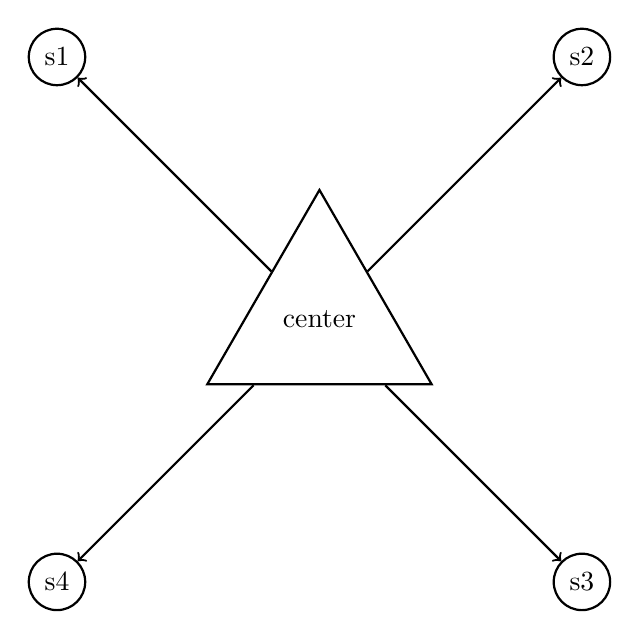
\begin{tikzpicture}\node[regular polygon,regular polygon sides=3,draw=black,align=center,line width=0.8pt] (0) at (5.833333333333333,10.0) {center};
\node[shape=circle,draw=black,align=center,line width=0.8pt] (1) at (9.166666666666666,13.333333333333334) {s2};
\node[shape=circle,draw=black,align=center,line width=0.8pt] (2) at (9.166666666666666,6.666666666666667) {s3};
\node[shape=circle,draw=black,align=center,line width=0.8pt] (3) at (2.5,6.666666666666667) {s4};
\node[shape=circle,draw=black,align=center,line width=0.8pt] (4) at (2.5,13.333333333333334) {s1};

\path [->,draw=black,line width=0.8pt] (0) edge node {} (1);
\path [->,draw=black,line width=0.8pt] (0) edge node {} (2);
\path [->,draw=black,line width=0.8pt] (0) edge node {} (3);
\path [->,draw=black,line width=0.8pt] (0) edge node {} (4);
\end{tikzpicture}
\end{document}